\documentclass{template/openetcs_article}
% Use the option "nocc" if the document is not licensed under Creative Commons
%\documentclass[nocc]{template/openetcs_article} 
\usepackage{rotating,url,color}
\graphicspath{{./template/}{.}{./images/}}
\begin{document}
\frontmatter
\project{openETCS}

%Please do not change anything above this line
%============================
% The document metadata is defined below

%assign a report number here
\reportnum{OETCS/WP2/D2.3.0~--~00/00}

%define your workpackage here
\wp{Work-Package 2: ``Requirements''}

%set a title here
\title{Preliminary Requirements for openETCS}

%set a subtitle here
%\subtitle{A template for short document. Adapted from report template.}

%set the date of the report here
\date{January 2013}

%define a list of authors and their affiliation here

\author{Sylvain Baro}
\affiliation{SNCF}
\author{Stanislas Pinte}
\affiliation{ERTMS Solutions}
  
% define the coverart
\coverart[width=350pt]{chart}

%define the type of report
\reporttype{Requirements}


\begin{abstract}
This document provides a preliminary view of the requirements for the openETCS project. 
It is meant to evolve after the initial release in order to provide the full requirement lists.
\end{abstract}

%=============================
%Do not change the next three lines
\maketitle
\tableofcontents
\listoffiguresandtables
\newpage
%=============================

% The actual document starts below this line
%=============================


%%%%%%%%%%%%%%%%%%%%%%%%%%%%%%%%%%%%%%%%%%%%%%%%%%%%%%%%%%%%%%
%%%              My macros (=> Sylvain Baro)               %%%
%%%%%%%%%%%%%%%%%%%%%%%%%%%%%%%%%%%%%%%%%%%%%%%%%%%%%%%%%%%%%%
\newcommand{\tbd}{\colorbox{cyan}{\%\%To Be Defined\%\%}}
\newcommand{\tbc}{\colorbox{cyan}{\%\%To Be Confirmed\%\%}}
\newcommand{\todo}[1]{\colorbox{cyan}{\%\%{#1}\%\%}}
\newlength{\origindent}

\newenvironment{issue}{
	\begin{quote}
	\begin{itshape}Open Issue. 
}{
	\end{itshape}
	\end{quote}
}

\newenvironment{comment}{
	\begin{quote}
	\begin{itshape}Comment. 
}{
	\end{itshape}
	\end{quote}
}

\newenvironment{justif}{
	\begin{quote}
	\begin{itshape}Justification. 
}{
	\end{itshape}
	\end{quote}
}
%% Requirements.


\newcounter{reqnum}
\setcounter{reqnum}{0}
\newcounter{subreqnum}
\newcounter{subsubreqnum}
\newlength{\partopbuf}
\newlength{\topbuf}

% Automated numbering versions of the macros
\newcommand{\req}[1]{\addtocounter{reqnum}{1} \setcounter{subreqnum}{0}
	\setlength{\partopbuf}{\partopsep}
	\setlength{\partopsep}{0pt}
	\setlength{\topbuf}{\topsep}
	\setlength{\topsep}{0pt}
	\begin{description}\item[{\small\reqt-X-\thereqnum}] #1\end{description}
	\setlength{\partopsep}{\partopbuf}
	\setlength{\topsep}{\topbuf}	
	}

\newcommand{\subreq}[1]{
	\addtocounter{subreqnum}{1} \setcounter{subsubreqnum}{0}
	\setlength{\partopbuf}{\partopsep}
	\setlength{\partopsep}{0pt}
	\setlength{\topbuf}{\topsep}
	\setlength{\topsep}{0pt}
	\begin{description}\addtolength{\leftmargin}{1cm}
	\item[{\small\reqt-X-\thereqnum.\thesubreqnum}] #1
	\addtolength{\leftmargin}{-1cm}\end{description}
	\setlength{\partopsep}{\partopbuf}
	\setlength{\topsep}{\topbuf}
}

\newcommand{\subsubreq}[1]{
	\addtocounter{subsubreqnum}{1}
	\setlength{\partopbuf}{\partopsep}
	\setlength{\partopsep}{0pt}
	\setlength{\topbuf}{\topsep}
	\setlength{\topsep}{0pt}
	\begin{description}\addtolength{\leftmargin}{1cm}
	\item[{\small\reqt-X-\thereqnum.\thesubreqnum.\thesubsubreqnum}] #1
	\addtolength{\leftmargin}{-1cm}\end{description}
	\setlength{\partopsep}{\partopbuf}
	\setlength{\topsep}{\topbuf}
}

% Fixed version of the commands
\newcommand{\reqfixed}[3]{\addtocounter{reqnum}{1} \setcounter{subreqnum}{0}
	\setlength{\partopbuf}{\partopsep}
	\setlength{\partopsep}{0pt}
	\setlength{\topbuf}{\topsep}
	\setlength{\topsep}{0pt}
	\begin{description}\item[{\small\reqt-#1-#2}] #3\end{description}
	\setlength{\partopsep}{\partopbuf}
	\setlength{\topsep}{\topbuf}	
	}

\newcommand{\subreqfixed}[4]{
	\addtocounter{subreqnum}{1} \setcounter{subsubreqnum}{0}
	\setlength{\partopbuf}{\partopsep}
	\setlength{\partopsep}{0pt}
	\setlength{\topbuf}{\topsep}
	\setlength{\topsep}{0pt}
	\begin{description}\addtolength{\leftmargin}{1cm}
	\item[{\small\reqt-#1-#2.#3}] #4
	\addtolength{\leftmargin}{-1cm}\end{description}
	\setlength{\partopsep}{\partopbuf}
	\setlength{\topsep}{\topbuf}
}

\newcommand{\subsubreqfixed}[5]{
	\addtocounter{subsubreqnum}{1}
	\setlength{\partopbuf}{\partopsep}
	\setlength{\partopsep}{0pt}
	\setlength{\topbuf}{\topsep}
	\setlength{\topsep}{0pt}
	\begin{description}\addtolength{\leftmargin}{1cm}
	\item[{\small\reqt-#1-#2.#3.#4}] #5
	\addtolength{\leftmargin}{-1cm}\end{description}
	\setlength{\partopsep}{\partopbuf}
	\setlength{\topsep}{\topbuf}
}

% Citation of the requirement

% Citation of the reference (for markup purpose)
\newcommand{\refreq}[1]{\textbf{#1}}

% Citation of the reference and text (for markup purpose)
% The purpose of this is to automatically replace the placeholder by the 
% full text. \fullrefreq{R-xxx}{} or \fullrefreq{R-xxx}{blabla} 
% will be replaced by \fullrefreq{R-xxx}{text of the R-xxx requirement} 
\newcommand{\fullrefreq}[2]{\textbf{#1}: \textrm{#2}}



\def\reqt{R-WP2/D2.3.0}
% Start here
\section{Introduction}
The purpose of this document is to enumerate the meta-requirements of the projects: \emph{i.e.} 
the requirements on the modeling, processes, toolchain. The purpose of this document is 
not to provide the system and safety requirements that will specify the model/software 
developed in the OpenETCS project.

The requirements found in the 50126 and 50128 are not rewritten here. The required plans for the 
project (see Sect. \ref{standards}) shall be written according to what is required in the standards,
then reviewed. Once this task is done, the plans will be the reference for the project.
In the meantime, one can refer to the standard, or to AeBT and TUBS presentations at WP2 Workshop.

This document is initiated as a preliminary requirement list, and will evolve during the project 
to be completed with all the requirements on the methodology
modelling, process, tool chain, and safety proof. The table herebelow sums up the area of responsibility
of the contributors of WP2 on these requirements.

\small
\begin{tabular}{|p{1.1cm}|p{1.8cm}|p{1.8cm}|p{3.2cm}|p{4.2cm}|}
\hline
Subtask ID & Requirements & Responsible & Major Participants & Participants \\
\hline
D2.3.1 & Set of requirements on modeling & TUBS & TUBS; SNCF; ALSTOM; Siemens & 
DLR; CEDEX?; Multitel?; Mitsubishi E.; Innovalia?; SQS? \\
\hline
D2.3.2 & Set of requirements on API & ALSTOM & SIEMENS; ALSTOM & 
ERSA?; SNCF; Fraunhofer;Innovalia?; SQS? \\
\hline
D2.3.3 &  Set of requirements on tools & ERTMS Solutions & SYSTEREL; CEA & 
\todo{STAN CONFIRM ACCORDING TO EFFORT- SNCF}; ERSA?; EclipseSource; ERTMS Solution; DLR; 
Mitsubishi E.; Innovalia?; SQS? \\
\hline
D2.3.4 & Set of requirements on V\&V & SNCF & SNCF; AEbT; ALSTOM; SIEMENS; DB; DLR & 
CEDEX?; Multitel?; Innovalia?; SQS? \\ 
\hline
\end{tabular}
\normalsize

\section{Reference documents}
\begin{itemize}
\item CENELEC EN 50126-1 --- 01/2000 --- \emph{Railways applications –- The specification and 
demonstration of Reliability, Availability, Maintenability and Safety (RAMS) –- Part 1: 
Basic requirements and generic process}
\item CENELEC EN 50128 --- 10/2011 --- \emph{Railway applications -- Communication, signalling and 
processing systems -- Software for railway control and protection systems}
\item CENELEC EN 50129 --- 05/2003 --- \emph{Railway applications –- Communication, signalling and 
processing systems –- Safety related electronic systems for signalling}
\item FPP --- \emph{Project Outline Full Project Proposal Annex OpenETCS} -- v2.2
\item SUBSET-026 3.3.0 --- \emph{System Requirement Specification}
\item SUBSET-076-x 2.3.y --- Test related ERTMS documentation
\item SUBSET-088 2.3.0 --- \emph{ETCS Application Levels 1 \& 2 - Safety Analysis}
\item SUBSET-091 2.5.0 --- \emph{Safety Requirements for the Technical Interoperability
of ETCS in Levels 1 \& 2}
\end{itemize}

\section{Conventions}
The requirements are prefixed by “R-zz-x-y”, and are written in a roman typeface, where ``R'' 
stands for ``Requirement'', ``zz'' identifies the source document,``x'' 
is the version number and``y'' is the identifier of the requirement. All the text 
written in italics is not a requirement: it may be a note, an open issue, an 
explanation of the requirements, or an example.

The placeholder “\todo{xxx}” is used to indicates that a paragraph or section is not finished, 
to be defined or to be confirmed.

\section{Glossary}
\begin{description}
\item[API] Application Programming Interface
\item[FME(C)A] Failure Mode Effect (and Criticity) Analysis
\item[I/O] Input/Output
\item[OBU] OnBoard Unit
\item[QA] Quality Analysis
\item[RBC] Radio Block Center
\item[RTM] RunTime Model
\item[SIL] Safety Integrity Level
\item[THR] Tolerable Hazard Rate
\item[V\&V] Verification \& Validation
\end{description}

\section{Goals}
\subsection{Goal 1: Formalization of the SRS in an executable formal and high level model}
The first goal of the project is to propose a formalization of a subset of the on-board subsystem,
as defined in the SUBSET-26. 

The purpose of the formalization is:
\begin{itemize}
\item to enhance the understanding of modelled subset;
\item to allow formal analysis of the modelled subset;
\item to be able to animate the model for testing an analyzing purpose;
\item to provide information on the completeness and soundness of the SUBSET-026; 
\item to point and document any contradiction or inconsistency of the SUBSET-026; 
\item to be used as a reference formal specification for the implementation of an OBU 
(by the OpenETCS project team and by industrial actors);
\item to be transformed in a later phase to lower-level source code, for the purpose of 
being executed or interpreted in an EVC subsystem;
\item \dots
\end{itemize}

In order to conduct this formalization, the tool chain and methodology defined (see Goal 2) 
shall be used.

The output of this goal is a formal specification that can be given to all railway actors, and 
if possible associated to SRS documents in the ERA database.

The final goal is that industrial actors work with this formal specification instead of 
natural language specification.

This formal specifications must be certifiable, but will not be certified as part of the project. 
\todo{STAN CONFIRM WITH SYLVAIN/PROJECT}

\subsection{Goal 2: Definition of a tool chain and process/methodologies for developing 
on onboard software that can fulfill the EN 50128 requirements}

These tools/methodologies must be certifiable, but will not be certified as part of the project.

By the combination of Goal 1 and 2, it should be possible for the industry to build an ETCS 
onboard software:
\begin{itemize}
\item By using OpenETCS model and proving the implementation satisfies the model;
\item By using the OpenETCS toolchain with their own model;
\item By using the OpenETCS model and toolchain.
\end{itemize}

The full safety process needed for the OpenETCS to be \emph{certifiable} according to CENELEC 50126
and 50128 shall be described in details. This safety plan will detail precisely which activities 
are required or not, why, and the choices that are made that allows to claim that safety is guaranteed.

Because the full design, development, validation and safety analysis process for a SIL4 OBU
is a huge task far beyond the project possibilities, the full safety activities will not be conducted
on the whole subsystem (see below). Nevertheless the safety process description shall be complete 
according to CENELEC requirements.

\subsection{Goal 3: Building an implementation of the subset of an onboard ETCS using the model and the 
tool chain defined in Goal 1 \& 2}

It is the demonstration that all the work done in the OpenETCS project is coherent, and that
the tool chain is operational.

\subsection{Goal 4: Define the safety properties at the model level}
In order to comply the CENELEC standards, it is necessary to conduct safety activities 
to identify errors and anomalies in the process. One important step for this is to define safety 
properties which are on the same level than the formal model.

These safety properties:
\begin{itemize}
\item will be used for the validation of the model itself;
\item will be used as reference proof obligations for the subsequent activies.
\end{itemize}

\begin{issue}
Is it realistic to expect such properties on the whole model? 
\end{issue}

\subsection{Goal 5: Provide a subset of the safety case}
Selected part of the safety process shall be applied (either by applying the full process on a small
subset of the development, or by applying a part of the activities on the whole project development).

\begin{issue}
This point has to be discussed. The purpose here is of course to demonstrate the feasability 
of the safety process, but I am not convinced that it proves anything if the whole process is 
not applied.
\end{issue}

\subsection{Goal 6: Promote OpenETCS}
Promote this work to push it to become a \emph{de facto} standard for the industrial actors, 
(like \emph{e.g.} the AUTOSAR standard in the automotive world).

\section{Project outline}
In order to pursue these goals, the development cycle for the project may be presented as follow. 

\textbf{Please note that this is just an outline of the activities, not the project plan, nor the 
Q\&A, nor the Validation plan. Also note that the activities needed for the toolchain are not
covered here.}

Fig. \ref{fig:main_process} shows the main part of the development process. This process may be seen
as a ``triple-V''. The smaller V corresponds to the development of the formal model. 

It starts by the SRS which is not part of the project (SUBSET-26), then outlines the boundaries and 
the applicable requirements from the SUBSET-26 that will be used in the formal model. 

The next step is the creation of the formal model itself. Because this model is executable, it can 
be validated as itself, thus the first ``closing branch'' of the V.

From the model can be derived some ``abstract'' code. The word ``abstract'' is used to emphasize that 
this code is not necessarily capable of running inside a full SIL4 platform. This code can be validated 
in the second ``closing branch'', possibly using some of the work done in the first branch. 

A project demonstrator may be derived from this code (or may be the ``abstract'' code itself).

The third ``closing branch'' corresponds to the production of code capable of running on a 
given SIL4 platform, and the associated validation activities. This is not part of the project.

The yellow boxes correspond	 to activities that should be covered completely in order to produce 
a certifiable product, but of which only a subset will be conducted in order to demonstrate the 
capabilities of the product.

\begin{figure}
  \centering
  \fbox{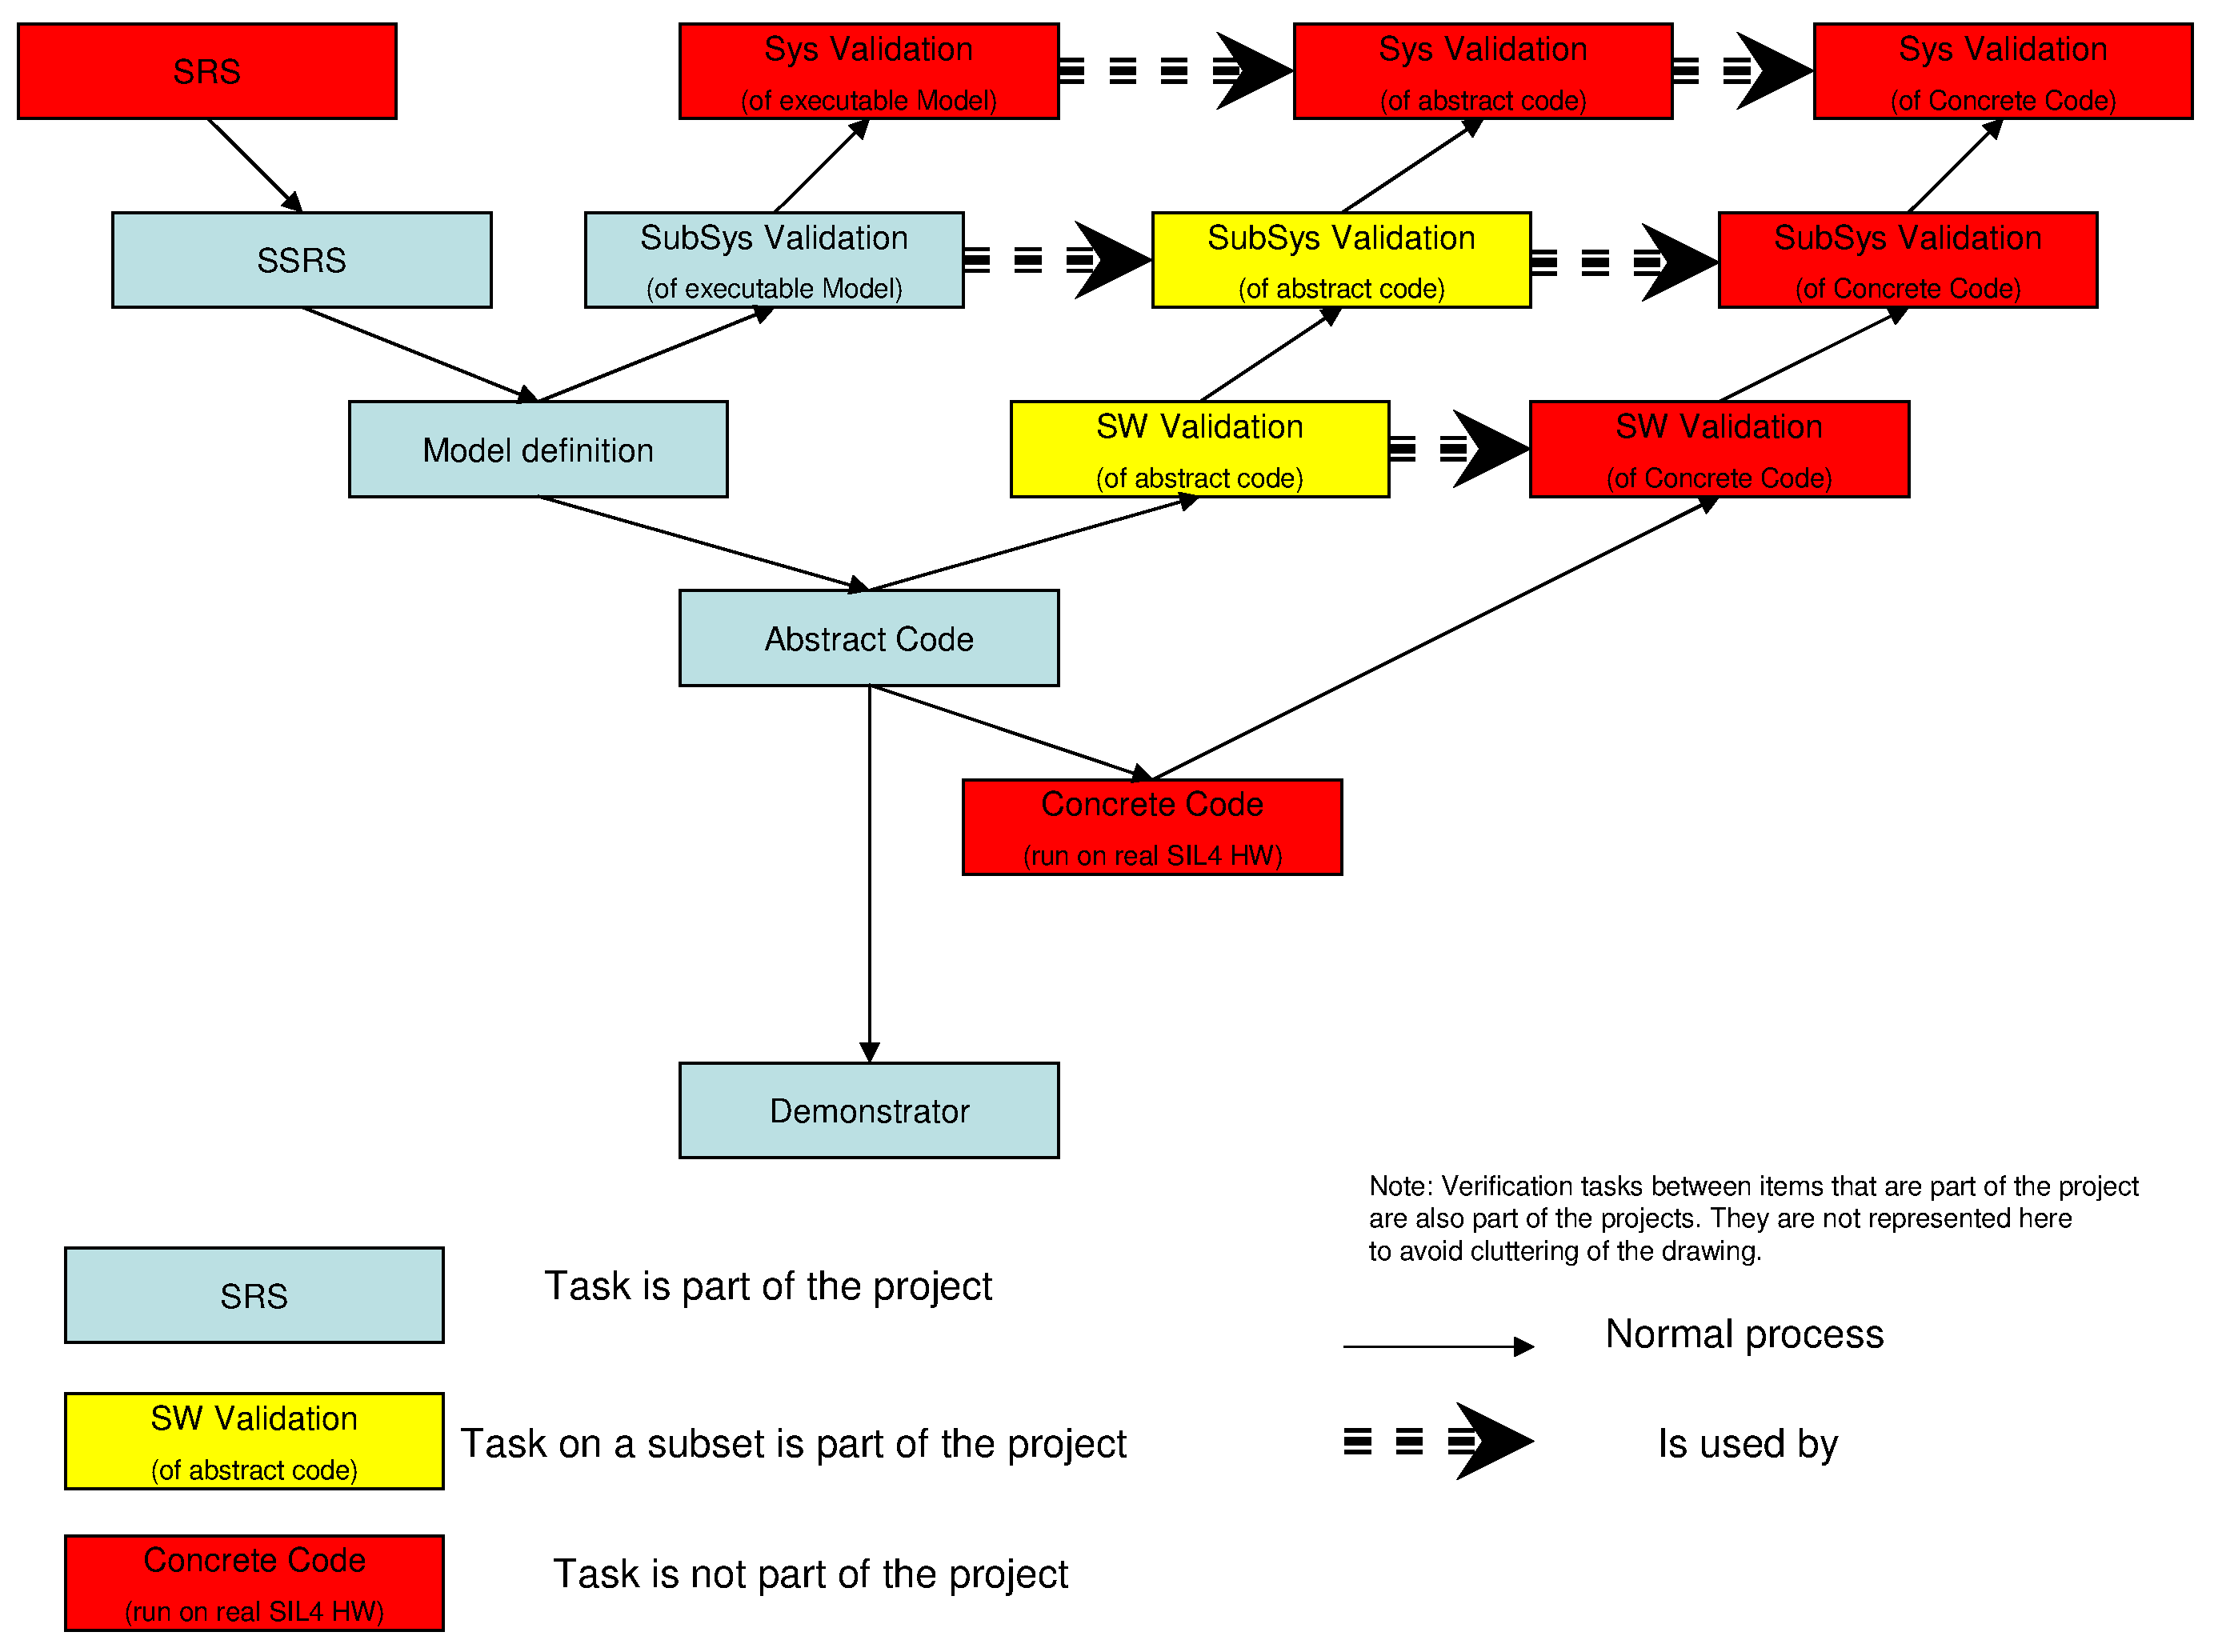
\includegraphics[scale=0.65]{Process1.png}}
  \caption{Main process}
  \label{fig:main_process}
\end{figure}

Fig. \ref{fig:safety_process} shows activities that are needed for the safety analyses. It should 
be considered in parallel of the descending branch of the V, but has been put on a separate diagram for
the sake of clarity.

High level safety properties are provided, which must be refined side-to-side with each step on the 
descending branch of the V. These properties are then used for the safety analysis of the model. The 
validation (safety analyses) boxes are yellow because the full activity will not be conducted. Only 
a subset of the safety properties will be proved.

\begin{figure}
  \centering
  \fbox{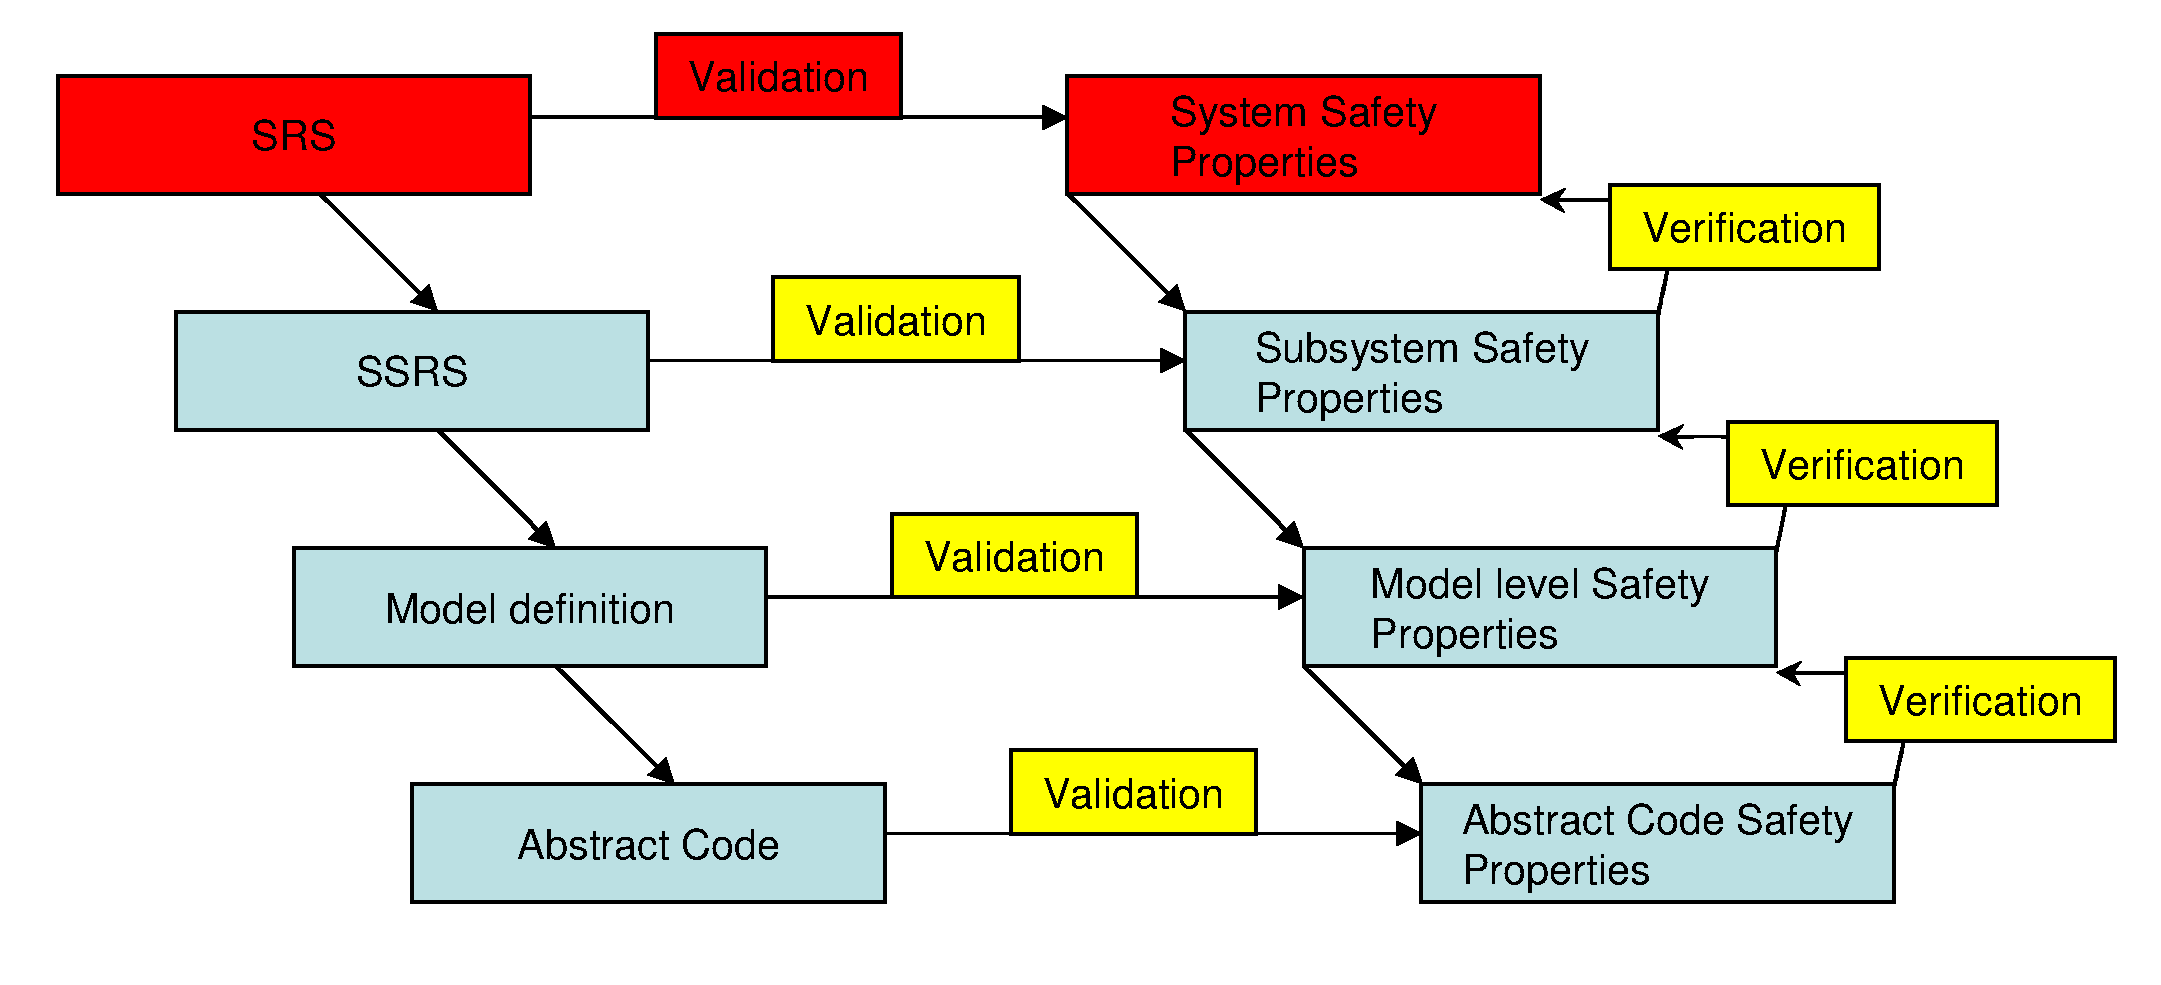
\includegraphics[scale=0.80]{Process2.png}}
  \caption{Safety analyses}
  \label{fig:safety_process}
\end{figure}

Regarding the process, WP2 shall issue (through this document) the requirements on V\&V, including
safety activities. From these requirements, WP4 shall propose the corresponding plans (Safety,
Verification and Validation). This plans will then be reviewed by WP2 to check conformance to the 
requirements. The reviewed plans will then be used as reference for the activities of the WPs.


\section{Requirements}
\subsection{Standards}
\label{standards}

\req{The project shall comply the CENELEC EN 50126 standard.}
\req{The project shall comply the CENELEC EN 50129 standard.}
\begin{comment}
These two requirements pulls some documentation issue (for example a project plan 
and a safety plan\,\footnote{Each plan is in the scope of the Work Package responsible for the 
corresponding tasks. \emph{I.e.} V\&V plan shall be issued by WP4.} which describe what to do in the 
context of an Open Source critical software), but it also pull other requirements (compliance to 
ISO~9001, skill of the people in contact with critical items). These points must be 
considered\,\footnote{The plan has to describe either how the requirement is applied in the context
of OpenETCS project, or why it is not needed.} in the QA Plan.
\end{comment}


\req{All software in the scope of the project shall comply the EN 50128 standard.}
\subreq{A QA Plan shall be issued and complied with.}
\subreq{The QA Plan shall describe the management of versions, OpenETCS baselines, 
connexion with ERTMS baselines, requirements\dots}
\subreq{A Verification plan shall be issued and complied with.}
\subreq{A Validation Plan shall be issued and complied with.}
\subreq{The techniques applied to the software will be compliant regarding the SIL.}
\subreq{All the output documents required by the EN~50126, EN~50128 and EN~50129 for 
each step of the lifecycle shall be issued, or their lack of shall be justified. A documentation plan shall be issued, and include the full list of documents.}
\subreq{The tools used shall be developed in order to be certifiable according to EN 50128.}

\begin{comment}
No requirement on the way of doing this. \emph{E.g.} to have a certified 
(certifiable?) code generator, two generators and comparison of the result, one
 generation and one verification chain\dots
 \end{comment}



\req{All Roles, responsabilities and more generally participators to any task (development, documentation, 
validation\dots) on any step of the project development shall be tracked, in particular
to show independence of the development and testing teams. The way of tracking shall be explained in
the QA Plan.}

\subsection{Runtime Model \& API}
\begin{figure}[h]
  \centering
  \fbox{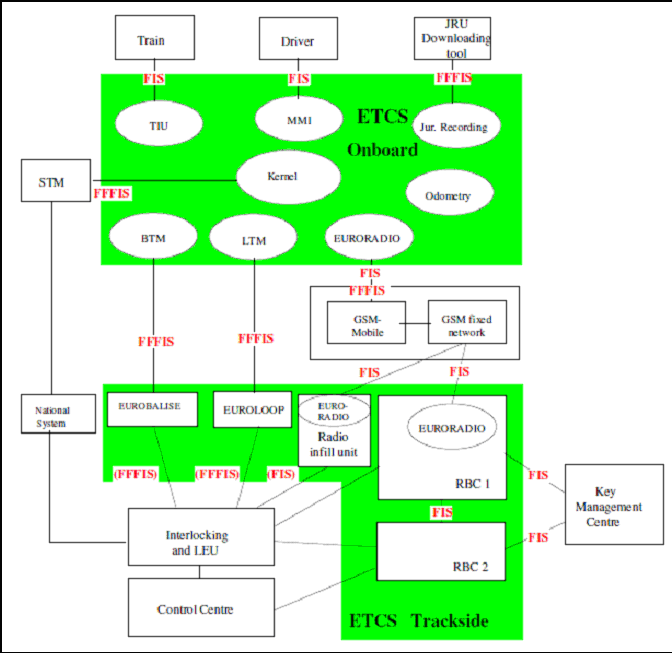
\includegraphics[width=4in]{archi}}
  \caption{Architecture}
  \label{fig:architecture}
\end{figure}

In order to avoid ambiguities, we will define the following.
\begin{description}
\item[Runtime model.] This is the abstract layer required to ``run'' the formal model. It shall provide
``hardcoded'' in the formalism part or all of the following (but not restricted to):
\begin{itemize}
\item memory management,
\item execution of state machines (or of the chosen formal objects), 
\item failures, 
\item communication between processes and concurrence. 
\end{itemize}
All these can be provided with or without safety properties. This corresponds in fact to the services 
provided by the ``abstract machine(s)'' which runs the models.
\item[API.]
 This is the functions/primitives required to complete the \emph{Runtime model}. It shall provide
the remaining of the features listed hereabove which are not provided by the Runtime model.

All these can be provided with or without safety properties.
\item[RTM/API.]
This corresponds to the Runtime Model \emph{plus} API. Therefore it should provide all the services
needed to emulate at abstract level the hardware platform that could run the software.
\item[Functional Architecture.] This corresponds to the functional boundaries between the ETCS KERNEL 
and the other functional components (JRU, DMI, Odometry, Eurobalise, Euroradio\dots). These boundaries
are described in the FIS or FFFIS. It also includes the parting of the KERNEL into different 
functions.
\end{description}

In the following requirements, we will not discriminate what is required from the API and from the 
RTM. This is the definition of these components that will allocate the requirements to the different 
parts. Hence we will only state requirements on the RTM/API.

\subsubsection{RTM/API}
\textbf{This chapter has to be completed by the leader of D2.3.2}

\req{The RTM/API model shall provide an abstraction layer of the hardware architecture.}
\req{The RTM/API shall make possible to refine the software into final code able to run 
on hardware complying the EN 50129 standard for the requested SIL.}

\req{The RTM/API shall allow discriminating Vital processing, data and I/O from Non Vital.}
\req{The RTM/API shall provide a way of communication between Vital processes and Non Vital processes.}

\begin{justif}
The purpose of these requirements is to be able to discriminate the safety part from the non 
safety part. It should be made possible to have it run on a proprietary architecture with both 
software on the same computer (with for example 2oo3, or coded monoprocessor) or on two 
different computers. One way of doing this, for example is to have some critical state 
machines with their data on one side, and the non critical part on the other side, with 
API channels to make them communicate.
\end{justif}

\begin{issue}Should it be done for just SIL4 and SIL0, or should there be all levels from SIL0 
to SIL4? It should be sufficient to distinguish only between safety and non safety, but an 
intermediate level could be useful (for SIL2 I/O for example). I have the feeling that it should not 
be more complicated to have one cluster of state machine per SIL, even if we only use SIL0 and SIL4.
\end{issue}

\req{The RTM/API shall allow to introduce failures for test purpose.}

\req{The RTM/API shall provide a way of reading configuration data (\emph{e.g.} constants,\dots)}

\req{The RTM/API shall provide an abstraction layer of the communication and interfaces 
with other components.}

\begin{justif}
Even if the FIS or FFFIS requires a specific protocol (\emph{e.g.} Profibus), this protocol will not 
be implemented in the high level model. It will be considered that low level communication issues are
taken into account (= emulated) by the RTM/API.
\end{justif}



\subsubsection{Model and Architecture}
\textbf{This chapter has to be completed by the leaders of D2.3.1 and D2.3.2}

\req{The model shall comply all OBU ETCS mandatory requirements, in the 
functional perimeter provided by the Functional Architecture.}

\subreq{The model shall comply the OBU part of SUBSET-026 version 3.3.0 or higher version.}

\subreq{The reference ETCS baseline shall be modified only by project decision, according
to the QA Plan.}
\subreq{All divergences against the chosen baseline shall be documented and tracked, according
to the QA Plan.}

\req{The model shall be as close as possible (in terms of level of abstraction) to the Subset-026 and shall yield as
few as possible “design choices”.}

\subreq{Complete bidirectional traceability between the model and the SRS shall be provided. }
\subreq{Each interpretation, ambiguity and inconsistency of the SRS shall be indicated precisely.}
\subreq{Each SRS requirement not formalized in the model (\emph{e.g.} allocated to RBC)
should be traced and justified.}
\subreq{Each missing SRS requirement, needed in the model (\emph{e.g.} any gap in the specification)
should be clearly identified and justified.}

\req{When the boundary of the formalized subsystem corresponds to a FIS or FFFIS, the Functional 
Architecture shall try to comply to it even when it is not mandatory.}

\req{The Functional Architecture shall split the KERNEL into independent functions.}
\begin{issue}
Should we stick to the SUBSET-026-4.5.2 function list?
STAN: Is this really needed at the model level? Is this really possible? A lot of the functions are going to relate to each other. 
For instance the braking curves depend on the MA processing that depends on location principles, etc.
According to our experience of modelling 33\% of Subset-026, it is impossible to split the kernel in independent functions. 
The only possible separation is in different namespaces, where fonctions are grouped (like BTM, ODO, Radio session, Speed supervision, ...)
However, one possible thing would be to track the dependencies between each namespace.
\end{issue}

\req{The Functional Architecture shall allow a universal method of adding functions, removing functions and overwriting functions (modularity and 
model extensibility). For instance, the model should allow the disabling of the SH mode.}

\todo{Design, Evolution, Validation, Transformation}


\section{Verification, Validation and Safety issues}
\textbf{This chapter has to be completed by the leader of D2.3.3}
\subsection{Safety}
\label{safety}
\begin{justif}
Side to side with the model (which should be a dynamic model), should lay a set of  
static safety properties on the model. The higher level properties will be provided 
by the WP2 (equivalent to a preliminary hazard analysis) from the SUBSET-91 document.

They will be refined by the safety analysis process (WP4) into properties of the same 
level than the model. The process of doing so shall be described in the Safety Plan.

This will provide Safety Properties on the model (or Dread Events). The lower level Safety Properties/
Dread Events shall address variables, state and interfaces used in the formal model.

Formal proof would then be used to prove that the OpenETCS model never enter a Dread State, 
as long as the other subsystem (RBC, communication layer\dots) fulfill their own safety properties
(axiom describing the environment).
\end{justif}

\req{A safety plan shall be provided and complied with.}
\req{The Functional Architecture shall identify the Vital and Non Vital functions.}
\req{The subsystem shall be compatible with the THR required in the SUBSET-091.}
\req{The safety analysis shall consider the Dread Event of the SUBSET-091, restricted to the
scope of the subsystem.}
\req{The model-level safety properties shall be written in a formal language.}

\tbc


\subsection{Verification and Validation}


\req{A V\&V plan shall be written and complied with.}

\begin{issue}Before stating the V\&V requirements, decisions should be taken regarding 
the safety issues raised in the previous section. The V\&V process will be heavily impacted
by the choice to do safety validation or not. 

If code is generated with refinement proof obligations, 
their will not be “verification testing”, but only “validation testing” 
(\emph{i.e.} functional tests).

If we use a formal method with automatic code generation, there is no need of unit testing. 
There would be only the need of validation (functional) tests (\emph{e.g.} Subset 076) and 
integration tests at the model level. Unit testing shall still be necessary at the code generator level.

\todo{Verification that the refinements of system design to software code is coherent?}\\

\todo{Verification that the proofs defined at system level design, are valids?}
\end{issue}

\tbc

\section{Language and formalism}
\textbf{This chapter has to be completed by the leader of D2.3.1}
Some of the requirements in this section could suit in the Tool Chain section, but for the sake 
of clarity I preferred to keep them near other language requirements.

\req{The model formalism shall be easily understandable by the domain experts.}
\req{The safety properties should be provided in a declarative, simple and formal language.}

\req{The formal model shall be transformable to others tools
(SCADE, Simulink, B tools, OpenETCS tool chain \todo{STAN is this a requirement on the language?} \dots}

\req{Formal specifications should be able to formalize:}
\subreq{State machines,}
\subreq{Time-outs,}
\subreq{Truth tables,}
\subreq{Arithmetics,}
\subreq{Braking curves,}
\subreq{Logical statements.}
\subreq{ERTMS Messages and fields.}

\begin{comment}
This requirement does not state that all these objects need to be \emph{first order objects} of
the language. It only state that it should be possible (easy?) to formalize and manipulate them.

It is to be noted that if (for example) braking curves are objects of the language, it shall be
proved that they are sound, and that the code generation for these objects is also sound.
\end{comment}

\req{The formal model shall be executable.}
\subreq{The formal model shall be executable in debug mode (step-by-step), allowing
inspection of states, variables and I/O.}
\subreq{The formal model shall support going back in time during a test, i.e. after having reached a certain step, to go backwards.}
\subreq{The formal model shall support what-if analysis, i.e. to change the value of any model variable during the execution of a test in order to measure its impact.}
\subreq{The formal model shall be self-explainable, i.e. shall be able to output its complete calculation tree
for complex functions, calling each other}
\subreq{The formal model shall support vizualization of the model elements activated during each step of a test}
\subreq{The formal model shall support importing and executing the Subset-076 test sequences}
\subreq{The environment shall be emulated by high level construction of the inputs.}

\req{The formal model should have a meta-model.}
\req{The formal model should have a meta-meta-model.}

\begin{justif}
``High level'' means that it will not be necessary to define bitwise the inputs at each cycle.
On the contrary, some automation will be available to define the behavior of the inputs.
\end{justif}

\req{It shall be possible to assert logical properties on the model (\emph{i.e. invariants}).}
\subreq{It shall be able to check the conformance of these properties at runtime.}
\subreq{It shall be able to prove the conformance of the model to these properties.}

\section{Tool chain}
\textbf{This chapter has to be completed by the leader of D2.3.2}

\req{The tool chain shall be composed only of Open Source components licensed under a license compatible with the EUPL license.}
\subreq{Closed source components may be used, but only if their use is not mandatory in the process, 
or if an open source counterpart is provided.}

\req{The tool chain shall be sufficiently robust to the management of the complete model, covering 100\% of the Subset-026.\footnote{As a reference, the Subset-026 includes roughly 3200 requirements applicable to the OBU.}}
\subreq{It shall allow modularity at any level (proof, model, software).}
\subreq{It shall support meta-model evolution.}
\subreq{It shall allow model-level refactoring, for instance rename model elements and move model elements.}
\subreq{It shall allow the management of documentation within the same tool.}
\subreq{It shall allow distributed software development.}
\subreq{It shall include an \emph{issue-tracking system}, in order to allow change management and 
errors/bugs management.}
\subreq{It shall offer suitable code-generation interface and services.}
\subreq{It shall allow to document/track the differences between the model and the ERTMS reference.}
\subreq{It shall support management of subsequent Subset-026 versions, as well as differences tracking between Subset-026 versions.}
\begin{justif}
In case where errors are found in the specification, or reducting choices are to be made in the 
model (\emph{e.g.} in case of non-determinism).
\end{justif}
\subreq{It shall allow concurrent version development, or be compatible with tools allowing
concurrent version development.}
\subreq{The version management tools shall use model-based version control, instead of text-based version control.\footnote{As explained in Towards software configuration management for unified models, \cite{Kogel:2008:TSC:1370152.1370158} "Traditional SCM systems operating on the abstraction of a filesystem and managing change at the granularity of textual lines are not adequate for these requirements. We propose a novel approach to SCM for unified models combining product versioning, operation-based deltas and change packages. To demonstrate feasibility we have implemented our approach in Sysiphus a suite of tools for collaborating over Software Engineering artifacts represented in a unified model."}}
\subreq{In particular, it shall be made easy\;\footnote{Especially in the case of a graphical language.}
to track the differences between two releases of a model and to manage conflicts.}
\subreq{In particular it shall allow to track the roles and responsabilities of each 
participant on a configuration item, at each step of the project lifecycle.}
\subreq{In particular, version management shall allow to track version of the safety properties 
together with the model.}

\req{The tool chain shall include support for the following graphical user interface facilities:}
\subreq{model syntax highlighting and auto-completion, for the parts of the model that are text-based}
\subreq{graphical representation of Subset-026 braking curves}	
\subreq{tree-based display of model elements}
\subreq{model animation and debugging}
\subreq{perspective management: offer in a single graphical user interface several interconnected views for SRS, model and tests.}

\req{The tool chain shall be platform independent, i.e. be portable accross windows, linux, mac, etc.}

\req{The tool chain shall allow traceability between:}
\subreq{the Subset-026 and the model, and vice-versa}
\subreq{the Subset-026 and the tests, and vice-versa}
\subreq{the model and the tests, and vice-versa}
\subreq{the documentation and the model}
\req{The tool chain shall allow traceability between the different layers of model and safety 
properties.}

\req{The tool chain shall provide the following reporting facilities:}
\subreq{detailed implementation metrics}
\subreq{detailed traceability reports}
\subreq{detailed model errors and warnings list}

\req{The tools used in the tool chain shall be able to cooperate, \emph{i.e.} the outputs of one 
tool will be suitable to be used as the inputs of the other tool.}

\req{The tool chain shall conform to 50128 requirements, for the corresponding SIL and tool class.}
\subreq{Each tool in the tool chain shall be classified among T1, T2 and T3}
\subreq{For T2 and T3 tools\,\footnote{T2: Tools contributing to the test or verification of the code 
or design 
\emph{e.g.} static analyzers, test generators\dots)\\ T3: tools contributing directly or indirectly
to the final code or data (\emph{e.g.} compilers, code translator\dots)}, the choice of tools shall be 
justified, and the justification shall
include how the tool's failures are covered, avoided or taken into account (ref. to EN 50128 6.7.4.2).}

\subreq{All T2 and T3 tools must be provided with their user manuals.}

\subreq{For all T3 tool, the proof of correctness  or the measure taken to guarantee the correctness 
of the output w.r.t. their specification and the inputs shall be provided.}
\subsubreq{\dots for data transformation,}
\subsubreq{\dots for software transformation (\emph{e.g.} translation, compilation\dots).}

\req{The tool chain shall allow to write, store and execute\emph{test cases} for the model.}

\req{The tool chain shall allow to generate test cases for the model.}
\begin{issue}
Is it really necessary? If we have formal proofs on the models, the tests should stay at a 
functional level. Therefore generated test cases should not be interesting in this context.
STAN: I confirm: if the test cases are generated based on the model, then any error
in the model shall cause the generation of incorrect test cases, and shall therefore not be detected. 
It is a real added value to have two independent parts in the model: one model part, and one test part, 
with the test part including test cases for all functions in the model. As these tests make up a
second implementation of the model, they enable a high-quality error detection in the model, 
also ensuring non-regression for the model. 
\end{issue}

\begin{issue}
TBD requirements on the prover. Should it verify De Bruijn's criterion\,\footnote{\emph{I.e.}
to be able to produce a proof tree that could be verified by a simple proof checker.}.
Should at least the proof tree be exportable and checkable in another tool? (if the proof
tree itself is mandatory).
\end{issue}

%%%%%%%%%%%%%%%%%%%%%%%%%%%

%% Bibliography
\nocite{*}
\bibliographystyle{unsrt}
\bibliography{req_synthesis}

% \begin{thebibliography}{9}

% \bibitem{lamport94}
  % Leslie Lamport,
  % \emph{\LaTeX: A Document Preparation System}.
  % Addison Wesley, Massachusetts,
  % 2nd Edition,
  % 1994.

% \end{thebibliography}

%===================================================
%Do NOT change anything below this line

\end{document}
